%%%%%%%%%%%%%%%%%%%%%%%%%%%%%%%%%%%%%%%%%%%%%%%%%%%%%%%%%%%%%%%%%%%%%%%%%%%%%%%%
% VisTacFusion — IEEE conference paper (ieeeconf class, ICRA/IROS style)
% Build: latexmk -pdf main.tex   (or scripts/compile.sh)
%%%%%%%%%%%%%%%%%%%%%%%%%%%%%%%%%%%%%%%%%%%%%%%%%%%%%%%%%%%%%%%%%%%%%%%%%%%%%%%%

\documentclass[letterpaper, 10pt, conference]{ieeeconf}

\IEEEoverridecommandlockouts   % needed for \thanks
\overrideIEEEmargins           % needed to meet printer requirements

\usepackage{graphicx}
\usepackage{amsmath}
\usepackage{amssymb}
\usepackage{booktabs}
\usepackage{multirow}
\usepackage{cite}              % sorted/ranged IEEE-style citation numbers
\usepackage{url}

% ---- convenience macros -------------------------------------------------------
\newcommand{\method}{VisTacFusion}
\newcommand{\todo}[1]{\textbf{\textcolor{red}{[TODO: #1]}}}
\usepackage{color}
\usepackage{subcaption}
\usepackage{tikz}
\usetikzlibrary{positioning, arrows.meta, calc, fit, backgrounds,
                 decorations.pathreplacing}

%%%%%%%%%%%%%%%%%%%%%%%%%%%%%%%%%%%%%%%%%%%%%%%%%%%%%%%%%%%%%%%%%%%%%%%%%%%%%%%%

\title{\LARGE \bf
\method{}: Asymmetric Visuo-Tactile Fusion for\\
Multi-Task Tactile Perception
}

\author{Xiangdong Huang$^{1}$% <-this % stops a space
\thanks{*This work was not supported by any organization.}%
\thanks{$^{1}$Xiangdong Huang is with \todo{affiliation}%
}

\begin{document}

\maketitle
\thispagestyle{empty}
\pagestyle{empty}

%%%%%%%%%%%%%%%%%%%%%%%%%%%%%%%%%%%%%%%%%%%%%%%%%%%%%%%%%%%%%%%%%%%%%%%%%%%%%%%%
\begin{abstract}
We present \method{}, a visuo-tactile multi-task model that jointly predicts
per-pixel depth, surface normals, and planar SE(2) object pose in the tactile
frame from a paired---but not pixel-aligned---RGB image and a vision-based
tactile image. Each modality is encoded by a frozen pretrained
encoder selected through systematic ablation: a tactile foundation model (T3)
for the gel image and a self-supervised vision model (MAE ViT-L) for RGB.
Features are combined by an asymmetric cross-attention trunk in which tactile
tokens serve as spatial queries while RGB enters only as read-only context
through a compact set of bottleneck tokens. Dense and pose prediction paths
are architecturally decoupled: the DPT decoder taps the tactile encoder
directly and receives 100\% of training steps, while modality dropout is
confined to the pose path, enabling a single set of weights to operate in
RGB+tactile, tactile-only, and RGB-only modes. This design yields a
controlled ablation of each modality's contribution: tactile alone matches
the fused model on depth (MAE 0.013) and normals ($1.21^{\circ}$) but
cannot resolve pose ($89.9^{\circ}$); RGB alone resolves pose
($2.18^{\circ}$) but lacks contact geometry (depth MAE 0.496); fusion
recovers both ($2.21^{\circ}$ pose, 0.013 depth MAE). Co-trained on
simulated and real data with frozen-encoder sim-to-real anchoring,
\method{} transfers zero-shot to real tactile sensors.
\end{abstract}

%%%%%%%%%%%%%%%%%%%%%%%%%%%%%%%%%%%%%%%%%%%%%%%%%%%%%%%%%%%%%%%%%%%%%%%%%%%%%%%%

\section{INTRODUCTION}

Contact-rich manipulation requires understanding both the global scene and the
local contact interface. An external RGB camera provides object identity,
orientation context, and coarse spatial layout, but is occluded precisely where
the gripper meets the object. A vision-based tactile sensor captures
high-resolution contact geometry---depth and surface normals at sub-millimeter
resolution---yet its field of view spans only the gel surface (${\sim}12$\,mm
after cropping). Neither modality alone is sufficient: tactile images of
geometrically symmetric objects (e.g.\ a circle, a square) are rotationally
ambiguous, while RGB lacks the contact detail needed for dense surface
reconstruction.

Prior work on visuo-tactile fusion typically assumes pixel-aligned image pairs
or operates separate, differently-sized models per modality configuration,
making it difficult to isolate the benefit of fusion from capacity
differences. Moreover, most methods share a single encoder for both
modalities, overlooking the growing availability of modality-specific
pretrained representations---tactile foundation models such as
T3~\cite{zhao2024transferable} and Sparsh~\cite{higuera2024sparsh}, and
self-supervised visual encoders such as MAE~\cite{he2022mae} and
DINOv2~\cite{oquab2023dinov2}---that offer stronger inductive biases when
matched to their respective domains.

\method{} addresses these gaps with three design decisions.
%
First, each modality is encoded by a \emph{frozen, modality-specific} encoder
selected through systematic ablation (T3 for tactile, MAE ViT-L for RGB);
freezing anchors sim-to-real transfer and guarantees that no encoder capacity
shifts between modality configurations.
%
Second, an \emph{asymmetric bottleneck fusion trunk} treats tactile tokens as
spatial queries and RGB as read-only key/value context, funnelled through a
small set of learnable bottleneck tokens. Because the output dimensionality
follows the query count, the decoder input is invariant to which modalities
are present.
%
Third, the dense prediction (DPT) and pose estimation paths are
\emph{architecturally decoupled}: the DPT decoder taps the tactile encoder
directly at its native 1024-dim multiscale features and trains on every step,
while modality dropout is confined to the pose path through the 768-dim
fusion trunk. This prevents dropout-induced dilution of dense supervision.

A single model trained with modality dropout supports three inference
modes---RGB+tactile, tactile-only, and RGB-only---with identical trainable
parameters, enabling a fair ablation of each modality's contribution.
Co-trained on simulated and real tactile data at an empirically optimized
ratio, \method{} transfers to real sensors without fine-tuning.

The contributions of this work are:
\begin{itemize}
\item An asymmetric bottleneck-attention architecture with decoupled dense and
      pose paths for fusing non-aligned RGB and tactile images, producing
      per-pixel depth, surface normals, and SE(2) pose in the tactile frame;
\item A systematic encoder ablation across six pretrained backbones, showing
      that modality-matched frozen encoders (T3 + MAE) outperform a single
      shared encoder;
\item A fair single-model ablation protocol---identical trainable parameters
      and decoder input across three input configurations---that isolates each
      modality's contribution and reveals complementary roles (tactile
      $\rightarrow$ dense geometry, RGB $\rightarrow$ pose disambiguation);
\item Sim-to-real transfer via frozen features and sim+real co-training,
      validated on real vision-based tactile sensors. \todo{sensor name}
\end{itemize}

% !TEX root = ../main.tex
\section{RELATED WORK}

\subsection{Vision-Based Tactile Sensing}
Vision-based tactile sensors such as GelSight~\cite{yuan2017gelsight} and
GelSlim~\cite{donlon2018gelslim} capture contact geometry through a
deformable elastomer illuminated by internal LEDs. Early depth reconstruction
methods relied on photometric stereo calibration; more recent approaches use
learned models to predict depth and surface normals directly from the gel
image~\cite{higuera2024sparsh}. Our work builds on this line but additionally
fuses an external RGB view for pose estimation.

\subsection{Visuo-Tactile Fusion}
\todo{Prior fusion work: MViTac~\cite{fu2024mvitac}, VITaL (CLIP-based);
symmetric fusion approaches (MBT~\cite{nagrani2021mbt}, shared
bottleneck averaging). Most assume aligned or object-centric fusion.
Contrast with our non-aligned, tactile-frame, asymmetric formulation
where tactile is the spatial anchor and RGB is read-only context.}

\subsection{Self-Supervised Representations for Touch and Vision}
Large-scale self-supervised pretraining has produced powerful frozen feature
extractors for both vision and touch.
DINOv2~\cite{oquab2023dinov2} and DINOv3~\cite{simeoni2025dinov3} learn
visual representations without labels;
MAE~\cite{he2022mae} reconstructs masked patches as a pretext task;
T3~\cite{zhao2024transferable} trains a sensor-specific encoder head atop a
shared ViT trunk on diverse tactile data;
Sparsh~\cite{higuera2024sparsh} applies DINOv2-style self-supervised learning
to tactile images.
We leverage these frozen encoders as a sim-to-real anchor: because the encoder
weights are never trained on our simulator, the feature space bridges the
domain gap without explicit domain adaptation.

\subsection{Dense Prediction and Multi-Task Learning}
The Dense Prediction Transformer (DPT)~\cite{ranftl2021dpt} reassembles
multiscale ViT features into dense maps via a convolutional decoder. We adopt
the DPT architecture for depth and surface normal prediction, and combine it
with a pose estimation head in a multi-task framework. Task balancing follows
grouped Kendall uncertainty weighting~\cite{kendall2018multi}, which
auto-balances losses within dense and pose groups independently.

\subsection{Sim-to-Real Transfer for Tactile Perception}
\todo{Sim-to-real for tactile: TACTO~\cite{wang2022tacto}, domain
randomization on gel images, frozen features as implicit domain bridge.
Our approach: heavy tactile photometric augmentation + frozen pretrained
encoders + sim+real co-training at optimized ratio. No explicit domain
adaptation (CORAL tried but did not improve over frozen-encoder baseline).}

% !TEX root = ../main.tex
\section{METHOD}

\begin{figure*}[t]
  \centering
  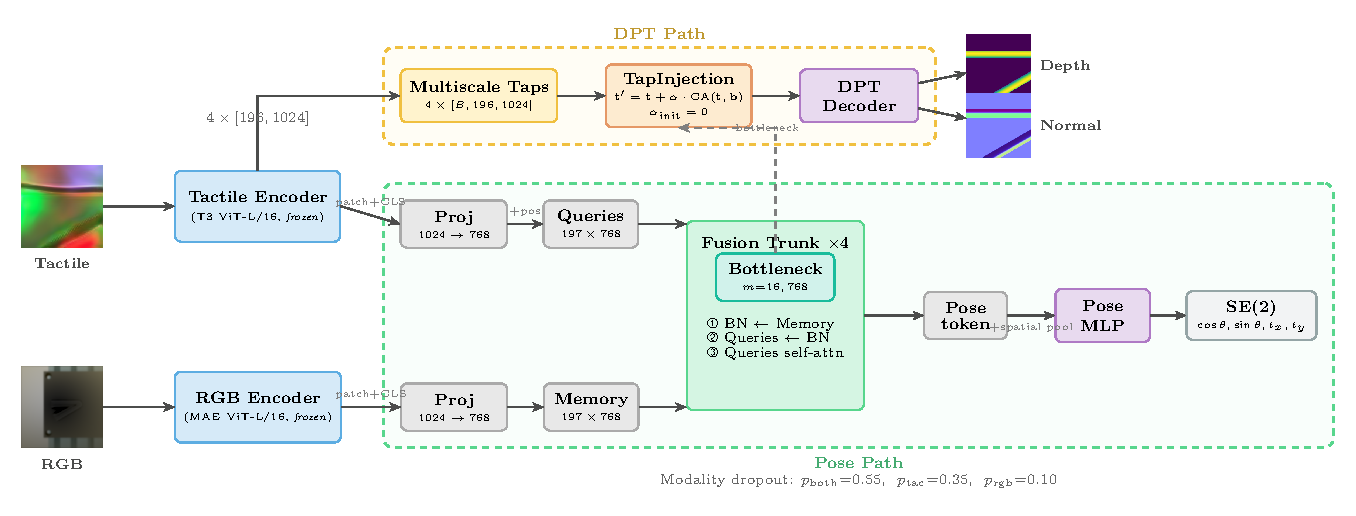
\includegraphics[width=\textwidth]{figures/architecture.pdf}
  \caption{\method{} architecture.
  %
  Frozen modality-specific encoders (T3 for tactile, MAE for RGB) extract
  features at 1024 dimensions. The \textbf{DPT path} (top): multiscale
  encoder taps feed directly into the DPT decoder for depth and normal
  prediction; optional RGB injection via ReZero-gated cross-attention
  ($\alpha$ init${}=0$) from the trunk's bottleneck adds visual context.
  %
  The \textbf{Pose path} (bottom): tactile tokens are projected to 768-dim
  and initialize 197 queries (196 spatial + 1 pose); RGB tokens form the
  read-only memory. A 4-layer asymmetric fusion trunk fuses them through 16
  learnable bottleneck tokens. The resulting pose token feeds an MLP that
  predicts SE(2) pose.
  %
  The decoder receives identical inputs regardless of which modalities are
  present, enabling a single model to serve three inference modes via
  modality dropout.}
  \label{fig:architecture}
\end{figure*}

\subsection{Transparency-Switchable Visuo-Tactile Sensor}
\label{sec:sensor}

\begin{figure}[t]
  \centering
  \todo{Fig.: (a) cross-section of the layer stack (photochromic layer,
  Solaris base, backing plate, UV LEDs, camera); (b) photo of the assembled
  prototype; (c) the same scene imaged in transparent and opaque mode.}
  \caption{Transparency-switchable sensor.
  (a)~Layer stack.
  (b)~Assembled prototype on the robot flange.
  (c)~Transparent mode (UV off) and opaque mode (UV on) views of the same
  contact.}
  \label{fig:sensor}
\end{figure}

GelSight-family sensors~\cite{yuan2017gelsight,donlon2018gelslim} coat the
gel with a permanent opaque reflective layer, which enables photometric
depth reconstruction but blocks the camera's view beyond the contact surface.
Prior dual-mode designs either keep the membrane semi-transparent and switch
by illumination contrast~\cite{hogan2021sts,athar2023vistac,prince2026mvptac},
or keep the gel transparent and track UV-excited
markers~\cite{wang2022spectac,yang2026transtac}, sacrificing part of the
reflective surface that dense reconstruction relies on.
We instead make the reflective layer itself switchable.
Building on the GelSlim~4.0~\cite{sipos2024gelslim4} body, we replace the
blue LEDs of its RGB illumination with UV LEDs and its coated gel with a
photochromic membrane that is transparent by default and turns opaque under
UV (Fig.~\ref{fig:sensor}).

The membrane is a two-layer Solaris\textsuperscript{TM} (Smooth-On) stack.
The 5\,mm base layer is mixed 1:1 by weight, vacuum-degassed, and cast in a
mold; it is optically clear once cured and serves as both the compliant
contact body and the transparent window.
The photochromic layer is spin-coated onto its outer face from 3\,g Solaris
mixed with 0.3\,mL of invisible UV-reactive ink (United Nuclear).
Because both layers are the same silicone, the film deforms with the base
rather than delaminating from it.
The photochromic layer is the outermost surface and contacts the object
directly, with no protective overlayer~\cite{prince2026mvptac}.
In opaque mode the reflective surface therefore coincides with the contact
surface, so the observed shading is produced at the exact geometry being
touched; in transparent mode the optical path contains only two
index-matched silicone layers, avoiding extra interface reflections in the
RGB view.
Despite the exposed surface, the membrane survived more than 40{,}000
contacts in durability testing without loss of switching function.

With UV off, the sensor operates in \emph{transparent mode} and the internal
camera images the external scene through the membrane, yielding $I_r$.
With UV on, the layer switches to an opaque reflective state within
\todo{xx}\,ms, and the remaining red and green LEDs illuminate it for
photometric tactile imaging, yielding $I_t$; the transition reverses
\todo{xx}\,s after UV is removed.
Both images come from the same Raspberry~Pi Zero camera module
(\todo{resolution}) through the same membrane, so they are paired by
construction but not pixel-aligned: the RGB view sees the object and its
surroundings beyond the gel, while the tactile view sees only the contact
patch.
\todo{active area diameter; housing; flange adapter; flex PCB role.}

\subsection{Data Collection}
\label{sec:data_collection}

Each object is rigidly mounted on a square platform attached to a
force--torque (FT) sensor.
Using the robot flange as a probe, we detect sequential edge contacts from
the FT signal, fit the four platform boundaries, and recover the platform
center and in-plane orientation, which define the object frame $\{O\}$ with
$0.1$--$0.2\,$mm in-plane accuracy.
\todo{Add ${}^{W}T_O$, ${}^{O}T_S$ equations if space permits.}

A KUKA LBR Med R820 arm then executes the same trajectory twice.
In Pass~1 the gel is removed and the camera captures a clean reference image
$I_{\text{clean}}^{(i)}$ with the robot pose $P_{\text{robot}}^{(i)}$ at each
waypoint.
In Pass~2 the switchable gel is installed and each waypoint yields a
transparent-mode image $I_{\text{trans}}^{(i)}$ (UV off), an opaque
non-contact background $I_{\text{bg}}^{(i)}$ (UV on), and a tactile image
$I_{\text{tac}}^{(i)}$ (UV on, in contact).
Repeating an identical trajectory maximizes spatial correspondence across
modalities.

\subsection{Problem Formulation}
Given a paired but non-pixel-aligned RGB image $I_r$ and vision-based tactile
image $I_t$, \method{} predicts, in the tactile frame: per-pixel depth $D$,
surface normals $\mathbf{N}$, and the object's planar pose
$(\theta, t_x, t_y) \in SE(2)$.

\subsection{Frozen Modality-Specific Encoders}
\label{sec:encoders}

Each modality is encoded by a frozen pretrained ViT-L encoder selected through
systematic ablation (Sec.~\ref{sec:encoder_ablation}): T3~\cite{zhao2024transferable}
for tactile and MAE~\cite{he2022mae} for RGB, both producing 1024-dim features
with 196 patch tokens ($14{\times}14$ grid at patch size 16).

Freezing serves two purposes.
First, it \emph{anchors sim-to-real transfer}: because the encoder weights are
never updated on simulated data, the feature space inherits the pretraining
distribution, bridging the sim-real domain gap without explicit adaptation.
Second, it ensures \emph{ablation fairness}: the trainable parameter count is
identical across all modality configurations, so no encoder capacity can shift
between modes.

Using separate, modality-matched encoders rather than a single shared backbone
yields an additional benefit: each encoder's inductive bias is tailored to its
input domain. T3's sensor-specific front-end captures gel-deformation patterns
that a generic vision encoder may overlook, while MAE's reconstruction-based
pretraining produces features well-suited to appearance-based recognition.

\subsection{Asymmetric Bottleneck Fusion Trunk}
\label{sec:trunk}

The fusion trunk operates at $D{=}768$ dimensions after a learned linear
projection from the encoder's native 1024-dim space. A separate
\texttt{BranchProjection} (linear + learned modality embedding) is applied to
each modality's tokens.

Tactile is the spatial anchor: its 196 projected patch tokens, augmented with
a learned spatial positional embedding, initialize the \emph{spatial queries};
its CLS token initializes the \emph{pose query} (197 queries total). RGB's
projected patch and CLS tokens form the read-only \emph{memory}
($197$ key-value tokens).

Each of the $L{=}4$ fusion layers applies three sequential attention steps:
\begin{enumerate}
\item \textbf{Bottleneck $\leftarrow$ Memory} (cross-attention, no FFN):
      $m{=}16$ learnable bottleneck tokens attend to the 197 RGB memory tokens,
      compressing RGB context into a compact representation.
\item \textbf{Queries $\leftarrow$ Bottleneck} (cross-attention + FFN):
      the 197 queries read from the $m$ bottleneck tokens, gating how much RGB
      information enters the tactile-anchored representation.
\item \textbf{Queries $\leftarrow$ Queries} (self-attention + FFN):
      queries refine amongst themselves.
\end{enumerate}
Because attention output length follows the query count, the trunk output is
always 197 tokens at 768-dim regardless of whether RGB is present. The
bottleneck tokens persist across layers (\emph{carry} mode), accumulating
progressively refined RGB context.

An optional per-object embedding $\mathbf{e}_{\mathrm{obj}} \in
\mathbb{R}^{768}$ is added to all 197 queries to provide object identity for
pose disambiguation across multiple objects.

\subsection{Decoupled Dense and Pose Paths}
\label{sec:decoupled}

The dense prediction and pose estimation paths are architecturally decoupled
to prevent modality dropout from diluting dense supervision.

\paragraph{DPT path.}
The DPT decoder~\cite{ranftl2021dpt} taps the \emph{tactile encoder}
directly at its native 1024-dim multiscale features, extracted at four
intermediate layers (layers 5, 11, 17, 23 of the 24-layer ViT). Each tap
receives a learned positional embedding before entering the DPT reassembly
($\text{Conv}_{1{\times}1}$: $1024 {\to} 256$, bilinear rescale) and
fusion-upsampling pipeline, producing depth ($C{=}1$) and surface normals
($C{=}3$) at the input resolution of $224{\times}224$.

Because the DPT path bypasses the fusion trunk, the pose-path modality
dropout never dilutes its tactile input: whenever the tactile image is
present (the \emph{both} and \emph{tactile} configurations, 90\% of steps)
the decoder sees pure tactile taps. In the RGB-only configuration the same
decoder falls back to the RGB encoder's multiscale taps, which is possible
because both encoders share the ViT-L token geometry (196 tokens, 1024-dim);
this yields a coarse shape prior rather than contact geometry
(Table~\ref{tab:modality_ablation}).

\paragraph{RGB injection via TapInjection.}
When RGB is available, visual context is optionally injected into the DPT taps
through a residual cross-attention mechanism with a ReZero gate:
\begin{equation}
  \mathbf{t}'_i = \mathbf{t}_i + \alpha_i \cdot
    \mathrm{CrossAttn}(\mathbf{t}_i,\, \mathbf{b})
  \label{eq:tap_inject}
\end{equation}
where $\mathbf{t}_i \in \mathbb{R}^{196 \times 1024}$ is the $i$-th encoder
tap, $\mathbf{b} \in \mathbb{R}^{16 \times 768}$ is the trunk bottleneck
(projected to 1024-dim for key/value), and $\alpha_i$ is a learnable scalar
initialized to zero. This ensures the DPT path starts as a pure
tactile-encoder pipeline and gradually learns to incorporate RGB context.
Injection is independently sampled per training step ($p = 0.5$), further
decoupling it from the pose path's modality dropout.

\paragraph{Pose path.}
After the fusion trunk, the pose token $\mathbf{p} \in \mathbb{R}^{768}$ and
mean-pooled spatial queries $\bar{\mathbf{s}} \in \mathbb{R}^{768}$ are
concatenated ($\mathbb{R}^{1536}$) and decoded by a 3-layer MLP to produce
$(\cos\theta, \sin\theta, t_x, t_y)$. The first two outputs are
L2-normalized to enforce unit-circle structure.

\subsection{Three Configurations, One Shared Model}
\label{sec:three_configs}

The model is trained with modality dropout: each step randomly samples one of
three input configurations with probabilities
$p_{\text{both}}{=}0.55$, $p_{\text{tactile}}{=}0.35$,
$p_{\text{rgb}}{=}0.10$.
%
At inference, these become three modes of the same trained weights:
\begin{itemize}
\item \textbf{RGB+tactile}: all three trunk steps run; DPT receives tactile
      taps with optional RGB injection.
\item \textbf{Tactile-only}: steps 1--2 are skipped (no RGB memory); only
      self-attention (step 3) refines the queries. DPT receives pure tactile taps.
\item \textbf{RGB-only}: learned mask tokens replace tactile queries; all
      three trunk steps run. DPT falls back to RGB encoder taps.
\end{itemize}
Importantly, the decoder input shape is identical in all three modes, so the
comparison is not confounded by architectural differences.

\subsection{Loss Functions and Training}
\label{sec:losses}

\paragraph{Task losses.}
Depth is supervised with MSE loss; surface normals with MSE loss; rotation
with $\mathcal{L}_{\text{rot}} = 1 - (\cos\hat\theta \cos\theta^*
+ \sin\hat\theta \sin\theta^*)$ (equivalent to $1 - \cos(\Delta\theta)$);
translation with L1 loss on $(t_x, t_y)$.

\paragraph{Grouped uncertainty weighting.}
Following~\cite{kendall2018multi}, we learn per-task homoscedastic uncertainty
terms, but group them into a \emph{dense} group (depth + normals) and a
\emph{pose} group (rotation + translation):
\begin{equation}
  \mathcal{L} = \lambda \sum_{i \in \text{dense}}
    \bigl(e^{-s_i}\mathcal{L}_i + \tfrac{1}{2}s_i\bigr)
  + \sum_{j \in \text{pose}}
    \bigl(e^{-s_j}\mathcal{L}_j + \tfrac{1}{2}s_j\bigr)
\end{equation}
where $s_i$ are learned log-variances and $\lambda$ is a fixed ratio between
groups. Grouping prevents pose improvements from starving dense gradients.

\paragraph{Training details.}
We train with AdamW ($\text{lr}{=}2 \times 10^{-4}$,
$\text{wd}{=}0.05$), cosine schedule with 1000-step linear warmup, for 150
epochs at batch size 64 per GPU on 2 GPUs (effective batch 128). Mixed
precision (fp16) and gradient clipping ($\|\cdot\| \leq 1.0$) are used
throughout. Only the projections, embeddings, bottleneck, fusion trunk, and
heads are trainable (${\sim}95$M of ${\sim}398$M total parameters).

\paragraph{Augmentation.}
Tactile images undergo heavy photometric augmentation---per-channel gain/bias,
directional gradients, residual noise, and Gaussian noise---to simulate sensor
variability across gel specimens and lighting conditions. RGB images receive
lighter, uniform-channel augmentation to preserve marker hue. Both modalities
undergo a fixed $1/\sqrt{2}$ center crop (eliminating border artifacts under
rotation augmentation) followed by a random gel-spin rotation
$\phi \sim \mathcal{U}(-180^{\circ}, 180^{\circ})$.

\paragraph{Sim+real co-training.}
\todo{Describe the simulated dataset (TACTO / other sim, objects, number of
samples) and the optimal real:sim ratio finding (1:2.7).}

\section{EXPERIMENTS}

\subsection{Experimental Setup}
\label{sec:setup}

\paragraph{Simulation data.}
We generate paired RGB-tactile training data in Blender for 20 objects across
12 sessions per object. Each sample consists of a tactile gel image, an
external RGB image, ground-truth depth (float32 \texttt{.npy}), and a
6-DOF pose annotation. A fixed $1/\sqrt{2}$ center crop yields an effective
$12.37$\,mm tactile field of view. All images are resized to
$224{\times}224$.

\paragraph{Real data.}
\todo{Describe your real sensor platform, data collection (5 objects,
session\_000), and how real samples are formatted to match sim.}

\paragraph{Metrics.}
We report: depth MAE and RMSE (contact region), normal angular error
(mean, degrees), pose rotation error (degrees, via
$\arccos(\cos\hat\theta\cos\theta^* + \sin\hat\theta\sin\theta^*)$),
and pose translation L1. All metrics are computed on the simulation
validation set (2400 samples, every 20th sample per session) unless
otherwise noted.

\paragraph{Baselines.}
We compare against: (1)~a shared-encoder baseline using a single frozen
DINOv3~\cite{simeoni2025dinov3} for both modalities with symmetric MBT-style
fusion; (2)~MViTac~\cite{fu2024mvitac}, a contrastive ResNet-18 baseline;
(3)~VITaL, a CLIP-pretrained ResNet-18 baseline with DPT decoder.
All baselines are trained with the same data, augmentation, and loss
configuration.

% -------------------------------------------------------------------------
\subsection{Does Fusion Beat Either Modality Alone?}
\label{sec:modality_ablation}

The central hypothesis is tested with the fair single-model protocol:
identical trainable parameters and identical decoder input across all three
configurations.

\begin{table}[t]
\caption{Modality ablation (one shared model, T3+MAE encoders, sim-only
training). Dense prediction is driven by tactile; pose by RGB; fusion
recovers both.}
\label{tab:modality_ablation}
\begin{center}
\begin{tabular}{lcccc}
\toprule
Config & \begin{tabular}{@{}c@{}}Depth\\MAE$\downarrow$\end{tabular}
       & \begin{tabular}{@{}c@{}}Normal\\(deg)$\downarrow$\end{tabular}
       & \begin{tabular}{@{}c@{}}Rot.\\(deg)$\downarrow$\end{tabular}
       & \begin{tabular}{@{}c@{}}Trans.\\L1$\downarrow$\end{tabular} \\
\midrule
RGB-only      & 0.496  & 12.67 & 2.18  & 0.008 \\
Tactile-only  & 0.013  & 1.21  & 89.94 & 0.205 \\
RGB+tactile   & \textbf{0.013} & \textbf{1.18}  & \textbf{2.21}  & \textbf{0.008} \\
\bottomrule
\end{tabular}
\end{center}
\end{table}

Table~\ref{tab:modality_ablation} reveals a striking complementarity.
Tactile-only achieves near-identical depth and normal accuracy as the fused
model (MAE 0.013, $1.21^{\circ}$), confirming that contact geometry is
overwhelmingly a tactile signal. However, tactile-only pose estimation is at
chance ($89.94^{\circ}$ $\approx$ uniform over $[-180^{\circ},
180^{\circ}]$), because geometrically symmetric objects cannot be
disambiguated from gel deformation alone.
Conversely, RGB-only recovers pose ($2.18^{\circ}$) via visual object
identity but cannot reconstruct contact depth (MAE $38{\times}$ worse).
Fusion inherits the strengths of both: the dense accuracy of tactile and
the pose disambiguation of RGB.

% -------------------------------------------------------------------------
\subsection{Encoder Ablation}
\label{sec:encoder_ablation}

We compare six frozen encoder pairings (tactile $\times$ RGB) while keeping
all other hyperparameters fixed. Training includes sim+real co-training.

\begin{table}[t]
\caption{Encoder ablation (sim+real co-training). Rotation and depth
evaluated in ``both'' (RGB+tactile) mode.}
\label{tab:encoder_ablation}
\begin{center}
\begin{tabular}{llcc}
\toprule
Tactile enc. & RGB enc. & Rot.\ (deg)$\downarrow$ & Depth MSE$\downarrow$ \\
\midrule
\textbf{T3}     & \textbf{MAE}    & \textbf{0.803} & 0.0195 \\
DINOv3 (shared) & DINOv3 (shared) & 0.812          & 0.0204 \\
SITR            & MAE             & 0.819          & \textbf{0.0159} \\
TVL             & MAE             & 0.844          & 0.0223 \\
T3              & DINOv3          & 1.481          & 0.0204 \\
T3              & CLIP            & 1.659          & 0.0208 \\
\bottomrule
\end{tabular}
\end{center}
\end{table}

Table~\ref{tab:encoder_ablation} shows that T3+MAE achieves the best pose
accuracy ($0.803^{\circ}$), outperforming the single shared DINOv3 baseline
($0.812^{\circ}$) despite using two separately pretrained encoders.
SITR+MAE achieves the best depth MSE, suggesting that calibration-aware
tactile encoders may better capture absolute surface geometry. The visual
encoder choice matters substantially for pose: MAE consistently outperforms
CLIP and DINOv3 as the RGB backbone, likely because its patch-level
reconstruction pretext captures the spatial appearance details needed for
orientation estimation.

% -------------------------------------------------------------------------
\subsection{Comparison with Baselines}
\label{sec:baselines}

\begin{table}[t]
\caption{Comparison with baselines (sim+real co-training, ``both'' mode).}
\label{tab:baselines}
\begin{center}
\begin{tabular}{lcc}
\toprule
Model & Rot.\ (deg)$\downarrow$ & Depth MSE$\downarrow$ \\
\midrule
\textbf{\method{} (T3+MAE)} & \textbf{0.803} & \textbf{0.0195} \\
Shared DINOv3 (MBT)         & 0.812          & 0.0204 \\
MViTac~\cite{fu2024mvitac}  & 1.203          & 0.1529 \\
VITaL                       & 2.271          & 0.0270 \\
\bottomrule
\end{tabular}
\end{center}
\end{table}

Table~\ref{tab:baselines} compares \method{} against three baselines trained
with the same data and losses. MViTac, which uses a contrastive ResNet-18,
achieves reasonable pose but poor depth reconstruction (MSE $7.8{\times}$
higher), highlighting the advantage of ViT-based multiscale features for
dense prediction. VITaL improves depth via its DPT decoder but trails in pose
accuracy ($2.271^{\circ}$ vs.\ $0.803^{\circ}$). The shared-DINOv3 baseline
with symmetric MBT fusion is a strong competitor; \method{}'s advantage comes
from the asymmetric design and modality-matched encoders.

% -------------------------------------------------------------------------
\subsection{Sim-to-Real Transfer}
\label{sec:sim2real}

\paragraph{Role of real data.}
Table~\ref{tab:real_ratio} reports the effect of varying the amount of real
data during co-training (with a fixed sim dataset).

\begin{table}[t]
\caption{Real data quantity ablation (T3+MAE, ``both'' mode).}
\label{tab:real_ratio}
\begin{center}
\begin{tabular}{rcc}
\toprule
Real samples & Rot.\ (deg)$\downarrow$ & Depth MSE$\downarrow$ \\
\midrule
0 (sim-only)    & 3.83  & \todo{--}  \\
25              & 2.126 & 0.0622 \\
100             & 1.029 & 0.0408 \\
300             & 0.825 & 0.0236 \\
all             & 0.886 & 0.0220 \\
\bottomrule
\end{tabular}
\end{center}
\end{table}

Performance improves rapidly with the first hundred real samples and saturates
around 300, with diminishing returns (and slight overfitting) beyond. The
optimal real-to-sim ratio is approximately 1:2.7.
\todo{Expand with your hardware/data-collection perspective on what makes
this ratio work (diversity of real contacts, etc.).}

\paragraph{Domain adaptation.}
We also evaluated explicit domain adaptation methods---CORAL feature alignment
and Fourier Domain Adaptation (FDA)---but neither improved over the
frozen-encoder baseline ($0.846^{\circ}$ and $0.845^{\circ}$ vs.\
$0.803^{\circ}$). This suggests that the frozen pretrained encoders already
provide sufficient domain invariance, and sim+real co-training handles the
residual gap.

\paragraph{Real sensor evaluation.}
\todo{Qualitative and quantitative results on real sensor data. Show
depth/normal visualizations and pose accuracy on real objects.}

% -------------------------------------------------------------------------
\subsection{Qualitative Results}
\label{sec:qualitative}

\todo{Figure: grid of depth/normal/pose predictions for representative
objects across the three input configurations (both, tactile-only, rgb-only),
on both sim and real data. Include failure cases (e.g.\ symmetric objects
under tactile-only).}

\section{CONCLUSIONS}

We presented \method{}, an asymmetric visuo-tactile fusion architecture for
multi-task tactile perception. By treating tactile as the spatial anchor and
RGB as read-only context through a compact bottleneck, and by decoupling the
dense prediction and pose estimation paths, \method{} reveals a clean
complementarity: tactile alone suffices for depth and normal reconstruction,
while RGB is essential for disambiguating object pose. A systematic encoder
ablation shows that modality-matched frozen encoders (T3 for tactile, MAE for
RGB) outperform shared backbones, and sim+real co-training at an optimized
ratio enables zero-shot transfer to real sensors without fine-tuning or
explicit domain adaptation.

\paragraph{Limitations.}
The current model is restricted to planar SE(2) pose under single-contact
assumptions. Depth and normal predictions are in the tactile frame only,
without integration into a global 3D reconstruction.

\paragraph{Future work.}
Extending to SE(3) pose with multi-finger contact, and using the fused
representation as input to downstream manipulation policies, are natural next
steps.


% \addtolength{\textheight}{-12cm}  % uncomment & tune on the page BEFORE the
                                    % last page to balance final columns

\section*{ACKNOWLEDGMENT}
\todo{acknowledgments}

%%%%%%%%%%%%%%%%%%%%%%%%%%%%%%%%%%%%%%%%%%%%%%%%%%%%%%%%%%%%%%%%%%%%%%%%%%%%%%%%

\bibliographystyle{IEEEtran}
\bibliography{references}

\end{document}
